
\chapter[On Curves which are the Schemes of
  Zeros of...]{On Curves which are the Schemes of
  Zeros of a Section of a rank Two Vector Bundle}\label{chap4}

\section{}\label{chap4:sec1}
 Let\pageoriginale $X$ be a scheme and $E$
a vector bundle on $X$. Suppose we are given a section of $E$. \ie an
injection $O_X\xrightarrow{s}E$. Then taking duals we get a morphism,
$\check{E}\longrightarrow O_X$. The cokernel of this map defines a
closed subscheme $Y$ of $X$, which we call the {\it scheme of zeroes
  of the section of $E$}. So we have an exact sequence,
$$
\check{E}\longrightarrow O_X\longrightarrow O_Y\longrightarrow 0
$$
\begin{figure}[H]
\centering
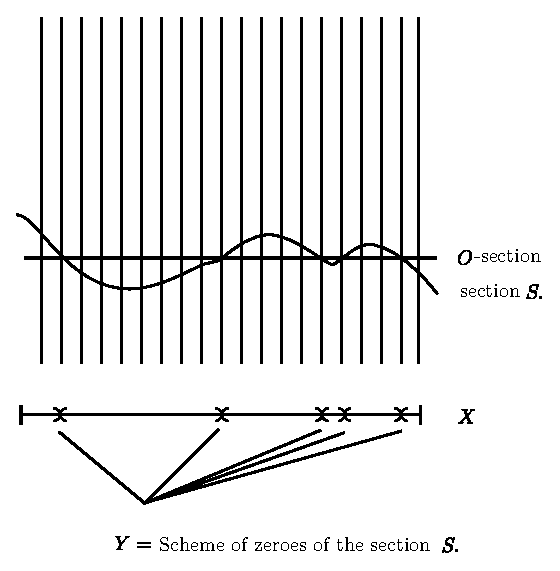
\includegraphics{figure/chap4-fig1.eps}

\medskip
{\bf Fig.~1}
\end{figure}

Now we prove a proposition by Serre, which gives a sufficient
condition for a closed sub-scheme of codimension two to be the scheme
of zeroes of a section of a rank two vector bundle.
\begin{Prop*}
{\bf (J-P. Serre):} Let\pageoriginale $Y$ be a regular, connected
scheme with dualising sheaf $\omega_Y$. Let $X$ be a closed sub-scheme
of $Y$, equidimensional, Cohen-Macaulay and of codimension two. Assume
the following conditions are satisfied:
\begin{itemize}
\item [a)] There exists a line bundle $L$ on $Y$ such that,
$$
\omega_X=L/X
$$
\item [b)] $H^2(Y,L^{-1}\otimes\omega_Y)=0$.
\end{itemize}

Then $X$ is the scheme of zeroes of a section of a rank two vector
bundle $E$ such that $\bigwedge\limits^2E\otimes\omega_Y=L$. 
\end{Prop*}

\begin{proof}
Let $J$ be the sheaf of ideals of $X$ in $Y$. If a vector bundle $E$
exists with the above properties, then we have the Koszul complex $0
\longrightarrow \bigwedge\limits^2\check{E}\longrightarrow\check{E}
\longrightarrow O_Y\longrightarrow O_X\longrightarrow 0$ with is
exact. So the sequence $0\longrightarrow\bigwedge\limits^2 \check{E}
\longrightarrow E\longrightarrow J\longrightarrow 0$ is exact. But we
want $\bigwedge\limits^2\check{E}$ to be equal to $L^{-1}\otimes
\omega_Y$. 

Thus we see that the problem is to find an extension of $J$ by
$L^{-1}\otimes\omega_Y$, which is a vector bundle \ie we want an
element of $\Ext^1(J,L^{-1}\otimes\omega_Y)$, which gives a locally
free extension. 

The spectral sequence for $\Ext$'s gives an exact sequence,
\begin{align*}
\Ext^1(J,L^{-1}\otimes\omega_Y) &\longrightarrow H^\circ(Y,
\underline{\Ext^1}(J,L^{-1}\otimes\omega_Y))\tag{A}\label{chap4:eqA}\\
&\longrightarrow H^2(Y, \underline{\Hom}(J,L^{-1}\otimes \omega_Y)).
\end{align*}

From the exact sequence,
$$
0\longrightarrow J\longrightarrow O_Y\longrightarrow
O_X\longrightarrow 0
$$
applying the functor $\Hom( \cdot , L^{-1}\otimes\omega_Y)$ and noting that
$\Ext^i(O_X,L^{-1}\otimes\omega_Y)$ is\pageoriginale zero if $i\neq 2$
(because $X$ is Cohen-Macaulay of codimension 2 in a regular scheme),
we see that 
\begin{gather*}
L^{-1}\otimes\omega_Y\simeq\underline{\Hom}(J,L^{-1}\otimes\omega_Y)\\ 
\intertext{and}
\Ext^1(J,L^{-1}\otimes\omega_Y)\simeq\Ext^2(O_X,L^{-1}\otimes\omega_Y). 
\end{gather*}

We know that $\underline{\Ext^2}(O_X'L_{-1}\otimes\omega_Y)=L^{-1}
\otimes\omega_X$ and by the assumption a) in the proposition,
$L^{-1}\otimes\omega_X=O_X$. Thus we see that
$\underline{\Ext^1}(J,L^{-1}\otimes\omega_Y)$ is a monogenic
$O_Y$-Module. This generator corresponds to a section $\eta$ of
$\underline{\Ext^1}(J,L^{-1}\otimes\omega_Y)$ and generates
$\underline{\Ext^1}(J,L^{-1}\otimes\omega_Y)$ at every point of $Y$.

Since $H^2(Y,\Hom(J,L^{-1}\otimes\omega_Y))$ is isomorphic to
$H^2(Y,L^{-1}\otimes\omega_Y)$ which is zero by assumption b) from
\eqref{chap4:eqA} we get that,
$$
\Ext^1(J,L^{-1}\otimes\omega_Y)\longrightarrow H^\circ(Y,
\underline{\Ext^1}(J,L^{-1}\otimes\omega_Y))
$$
is surjective. So there is an element of $\Ext^1(J,L^{-1}\otimes
\omega_Y)$ which maps onto $\eta$. Let $\check{E}$ be the extension
corresponding to this element. We will show that $\check{E}$ is
locally free.

We prove the following: Let $\eta$ be a section of $\underline{\Ext^1}
(J,L^{-1}\otimes\omega_Y)$ coming from
$\Ext^1(J,L^{-1}\otimes\omega_Y)$. The corresponding extension $G$ is
free at a point $y$ in $Y$ if and only if the image of $\eta$ in
$\Ext_{O_Y,y}^1(J_y(L^{-1}\otimes\omega_Y)_y)$ generates it as an
$O_{Y,y}$-module. This will prove our assertion that $\check{E}$ is
locally free. Assume $G$ is free at $y$. So we have an exact sequence,
$$
0\longrightarrow(L^{-1}\otimes\omega_Y)=O_{Y, y}\longrightarrow G_y=
O_{Y,y}\oplus O_{Y,y}\longrightarrow J_y\longrightarrow 0,
$$
which gives rise to an exact sequence,
$$
O_{Y,y}=\Hom_{O_{Y,y}}(O_{Y,y},O_{Y,y})\longrightarrow\Ext_{O_{Y,y}}^1
(J_y,O_{Y,y})\longrightarrow 0.
$$\pageoriginale

Since image of $\eta$ corresponds to image of the identity of
$O_{Y,y}$ in $\Ext_{O_{Y,y}}^1(J_y,O_{Y,y})$ we see that image of
$\eta$ generates it. Conversely let image of $\eta$ generate
$\Ext_{O_{Y,y}}^1(J_y,O_{Y,y})$ and let $G_y$ be the corresponding
extension. 

From the exact sequence,
$$
0\longrightarrow O_{Y,y}\longrightarrow G_y\longrightarrow J_y
\longrightarrow 0
$$
we see that the assumption implies, $\Ext^1(G_y,O_{Y,y})=0$. Since $Y$
is regular and $X$ is Cohen-Macaulay of codimension 2, we see that,
(Projective dimension of $G_y)\leq 1$. So for any $O_{Y,y}$-module
$N, \Ext^1(G_y,N)=\Ext^1(G_y,O_{Y,y})\otimes N=0 \,\ie\, G_y$ is
projective and hence free. 

Thus $\check{E}$ is locally free. From the exact sequence,
$0\longrightarrow L^{-1}\otimes\omega_Y\longrightarrow\check{E}
\longrightarrow J\longrightarrow 0$, one sees by additivity of ranks,
that rank $\check{E}$ is 2. We have an exact sequence,
$$
0\longrightarrow L^{-1}\otimes\omega_Y\longrightarrow\check{E}
\longrightarrow O_Y\longrightarrow O_X\longrightarrow 0.
$$

The fact that the Koszul complex
$$
0\longrightarrow\bigwedge\limits^2\check{E}\longrightarrow\check{E}
\longrightarrow O_Y\longrightarrow O_X\longrightarrow 0.
$$
is\pageoriginale also exact implies that $\bigwedge\limits^2\check{E}
\simeq L^{-1}\otimes\omega_Y$. So $X$ is the scheme of zeroes of a
section of the rank two vector bundle $E$ with $\bigwedge\limits^2E
\otimes\omega_{Y/X}=\omega_X$. 
\end{proof}

\begin{REM*}
Conversely if $X$ and $Y$ are as in the proposition and if $X$ is the
scheme of zeroes of a section of a rank two vector bundle $E$, then
one can see that a) is satisfied \ie $\bigwedge\limits^2E\otimes
\omega_{Y/X}=\omega_X$. But b) may not be satisfied.
\end{REM*}

\begin{Coro*}
Let $Y=\Spec R$ where $R$ is a regular ring. If $X$ and $Y$ satisfy
the conditions in the proposition (note that $H^2(Y,\cdotp)=0$, since
$Y$ is affine.) then $X$ is a local complete intersection. In
addition, if projectives are free over $R$, then $X$ is a complete
intersection. 

As an interesting corollary to Serre's proposition, we will prove the
following: 
\end{Coro*}

\begin{THM*}
{\bf (G. Horrocks)}. Give any pair of integers $C_1$ and $C_2$, there
exists an indecomposable rank two vector bundle $E$ on $\mathbb{P}_k^3
(k$ infinite) such that $C_1(E)=C_1$ and $C_2(E)=C_2$ (where $C_i(E)$
denote the $i^{th}$ Chern number of $E$) if and only if $C_1C_2=0\mod
2$ 

We recall some definitions and properties of Chern numbers: Let $E$ be
a vector bundle on $\mathbb{P}^3$ of rank 2. Let $X$ be a scheme of
zeroes of a section of $E$.

Then $\omega_X=O_X(C_1(E)-4)$ and $C_2(E)=d^\circ X$. 

We also note that,
\begin{align*}
C_1(E(n)) &= C_1(E)+2n\\
C_2(E(n)) &= C_2(E)+n C_1(E)+n^2,
\end{align*}\pageoriginale
and $C_1(\check{E})=-C_1(E)$. 
\end{THM*}

\begin{proof}
(of the theorem). First we will show that $C_1C_2=0 (\mod 2)$ is a
  necessary condition for any vector bundle of rank two on
  $\mathbb{P}^3$. Let $E$ be any vector bundle of rank 2 on
  $\mathbb{P}^3$. Since $C_1(E)C_2(E)-C_1(E(n)).\break C_2(E(n))=0 (\mod 2)$
  for any $n$, it is sufficient to show for large $n$. Hence we can
  assume that $E$ has a smooth section, say $X$. Then
$$
\Omega_X^1=\omega_X=O_X(C_1(E)-4).
$$

By Riemann-Roch, $\deg\Omega_X^1=2g-2$, and
$\deg\omega_X=C_2(E)(C_1(E)-4)$. So $C_1(E). C_2(E)=0 (\mod 2)$. 

We will now construct indecomposable vector bundles of rank 2 with
given Chern numbers. 
\begin{itemize}
\item [I] Let $a>0$ be any integer and $m_1,m_2\ldots m_r$ be integers
such that $0<m_i<a$. Then there exists a vector bundle $E$ of rank
2. Such that $C_1(E)=a$ and $C_2(E)=\sum\limits_{i=1}^r m_i(a-m_i)$
and an exact sequence,
$$
0\longrightarrow O_{\mathbb{P}^3}(-a)\longrightarrow E\longrightarrow
O_{\mathbb{P}^3}\longrightarrow O_X\longrightarrow 0
$$
\ie $X$ is the scheme of zeroes of a section of $E$. We\pageoriginale
will prove this by induction on $r$. If $r=1$, we take
$E=O(m_i)+O(a-m_i)$. Assume we have proved this upto $(r-1)^{th}$
stages so we have a vector bundle $E$ such that 
$$
C_1(E)=a, C_2(E)=\sum\limits_{i=1}^{r-1}m_i(a-m_i)
$$
and an $X$ which is the scheme of zeroes of a section of $E$.

\noindent So $\omega_X=O_X(C_1(E)-4)=O_X(a-4)$ and 
$$
d^\circ(X)=C_2(E).
$$

One can easily see that the zeroes of a generic section of $O(m_r)
\oplus O(a-m_r)$ does not meet $X$. So let $X_1$ be such a
scheme. Then $\omega_{X_1}=O_{X_1}(a-4)$ and $d^\circ
X_1=m_r(a-m_r)$. From this we see that $X\cup X_1$ is locally a
complete intersection and $\omega_{X\cup X_1}=O_{X\cup X_1}(a-4),
d^\circ(X\cup X_1)=C_2(E)+m_r(a-m_r)=\sum\limits_{i=1}^rm_i
(a-m_i)$. Serre's proposition assures that $X\cup X_1$ is the scheme
of zeroes of a section of a rank two vector bundle, say $F$. Then
$C_1(F)=a$ and $C_2(F)=\sum\limits_{i=1}^rm_i(a-m_i)$ and we have a
section as required. 
\item [II] By the above construction, if $r\geq 2$, then the
  corresponding vector bundle $E$ is indecomposable. If $r\geq 2$,
  then by construction, there exists a section, the scheme of zeroes
  $X$ of which has more than one connected component. Let $X$ be the
  scheme of zeroes of any section. Then one verifies from the exact
  sequence corresponding to the section that 
$$
\dim H^1(\mathbb{P}^3,\check{E})=\dim H^\circ(X,O_X)-1.
$$

If $X$ has more than one connected component we see that\break $\dim H^1
(\mathbb{P}^3,\check{E})\geq 1.\, \ie \, H^1(\mathbb{P}^3,\check{E})\neq
0$. If $E$ is decomposable, then so is $\check{E}$ and then
$H^1(\mathbb{P}^3, \check{E})=0$. So if $r\geq 2$, we see that $E$ is
indecomposable. 

We\pageoriginale denote by $\Delta(E)$, then number,
$C_1(E)^2-4C_2(E)$. Note that $\Delta(E(n))=\Delta(E)$. If $C_1$ and
$C_2$ are two integers with $C_1C_2\equiv 0\mod 2$, we see that,
$C_1^2-4C_2\equiv 0(\mod 4)$ if $C_1$ is even and $\equiv 1(\mod 8)$
if $C_1$ is odd.
\end{itemize}
\end{proof}

\begin{lem*}
Let $n$ be a positive integer $\equiv 0(\mod 4)\; \text{or} \; \equiv
1(\mod 8)$. Then there exists positive integers $a,m_1$ and $m_2$ such
that, $0<m_i<a$ and $n=a^2-4. \sum\limits_{i=1}^2m_i(a-m_i)$. 
\end{lem*}

\begin{proof}
Because of the conditions on $n$ there exists a positive integer $N$
such that $N^2=n+8m_1m_2$ where $m_i$'s are some positive
integers. Then take $a=2(m_1+m_2)+N$. 
\begin{itemize}
\item [III] Let $C_1$ and $C_2$ be any two integers such that
  $C_1C_2=0 \mod 2$. Now we will construct an indecomposable vector
  bundle of rank 2, whose chern numbers are $C_1$ and $C_2$. 

By the above lemma, we have an expression, $C_1^2-4C_2=a^{2.}-4
\sum\limits_{i=1}^r m_i(a-m_i)$. With $0<m_1<a$ and $r\geq 2$. So by
our construction we have a vector bundle $E$ of rank two such that
$C_1(E)=a$ and $C_2(E)=\sum\limits_{i=1}^rm_i(a-m_i)$. Since $r\geq 2
E$ is indecomposable. $C_1-a=2m$ for some $m$. Now
$C_1(E(m))=a+C_1-a=C_1$ and
$\Delta(E(m))=\Delta(E)=C_1^2-4C_2$. Therefore $C_2(E(m))=C_2$ and
$E(m)$ is indecomposable. 
\end{itemize}
\end{proof}

\section{Thickening in a Normal Direction}\label{chap4:sec2} 
Let $Y$ be any regular scheme and $X$ a closed subscheme of $Y$ which is a
local complete intersection. So the conormal bundle $N_X$ is a vector
bundle over $X$.

Let $L$ be any line bundle over $X$ and let $N_X\longrightarrow L$ be
any surjection. Then we have a diagram, 
\[
\xymatrix{
0 \ar[r] &  N_X \ar[d] \ar[r]  & O_X\\
& L \ar[d] &\\
& 0 &
}
\]\pageoriginale
where $O_{X-1}=O_{Y/I^2}, I$, the ideal sheaf of $X$. Let $O_Z$ be the
push out. So $O_Z$ is the structure sheaf of a scheme $Z$ which is
closed in $Y$ and topologically isomorphic to $X$. So we have
commutative diagram,
\[
\xymatrix{
0\ar[r] & N_X\ar[d] \ar[r] & O_{X_1} \ar[d] \ar[r] & O_X \ar @{} [d]
|{\|} \ar[r] & 0\\
0 \ar[r] & L\ar[d] \ar[r] & O_Z\ar[d]\ar[r] & O_X\ar[r] & 0\\
& 0 & 0 & & 
}
\]
\begin{def*}
$Z$ {\it is defined as the thickening of} $X$ {\it in the direction of
the quotient} $L$. 
\begin{figure}[H]
\centering
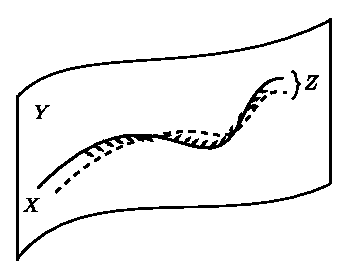
\includegraphics{figure/chap4-fig2.eps}

\medskip
{\bf Fig. 2}
\end{figure}
\end{def*}

\section[Curves which are Zeros]{Curves which are Zeros of Sections of
  Rank Two Vector Bundels in 3-Space}\label{chap4:sec3}
In\pageoriginale this section we will prove that curves in a smooth
quasiprojective scheme of dimension 3, which are local complete
intersection are\break schemes of zeroes of a section of a rank two vector
bundle. 

We start with a proposition due to R. Fossum:
\begin{Prop*}
Let $A$ be a local ring which is Cohen-Macaulay. Let $\omega_A$ be its
dualising sheaf. Let $B$ be any algebra extension of $A$ by $\omega_A$
with square of $\omega_A$ zero. Then $B$ is Gorenstein.
\end{Prop*}

\begin{proof}
We have an exact sequence of $B$-modules,
$$
0\longrightarrow\omega_A\longrightarrow B\longrightarrow
A\longrightarrow 0.
$$

Let $B$ be the quotient of a regular local ring $R$. One can assume
without loss of generality that $B$ is complete. Then $A$ is also a
quotient of $R$,  in a natural way. Codimension of $B$ and $A$ in $R$
are equal, say $r$. Let $\dim R=n$. Then $\Ext_R^i(A,R)=0$ for $i\neq
n-r$ 
$$
=\omega_A\quad i=n-r.
$$

Since $\omega_A$ is the dualising sheaf of $A$, we see that,
\begin{align*}
\Ext_R^i(\omega_A,R) &= 0\quad\text{for}\quad i\neq n-r\\
&= A\quad\text{for}\quad i=n-r. 
\end{align*}

Thus applying the functor $\Hom_R(.,R)$ to the above exact sequence,
we see that,
$$
\Ext_R^i(B,R)=0,\quad\text{for}\quad i\neq n-r.
$$

Therefore $B$ is Cohen-Macaulay. Hence $\Ext_R^{n-r}(B,R)=\omega_B$,
the dualising sheaf of $B$. So we get an exact sequence, 
$$
0\longrightarrow\Ext_R^{n-r}(A,R)\longrightarrow\Ext_R^{n-r}(B,R)
\longrightarrow\Ext_R^{n-r}(\omega_A,R)\longrightarrow 0
$$
\ie\pageoriginale $0\longrightarrow\omega_A\longrightarrow\omega_B
\longrightarrow A \longrightarrow 0$ is exact.

\noindent If $x$ in $R$ is a non-zero divisor in $A$, then it is also
a non-zero divisor in $\omega_A$. Hence it is also a non-zero divisor
in $B$ and $\omega_B$. Going modulo such an $x$, we get an exact
sequence.
$$
0\longrightarrow\omega_{A/x\omega_A}\longrightarrow
\omega{B/x\omega_B}\longrightarrow A/_{xA}\longrightarrow 0.
$$

But since $\omega_{A/x\omega_A}=\omega_{A/x A}$ and
$\omega_{B/x\omega_B}=\omega_{B/xB}$ we have 
$$
0\longrightarrow\omega_{A/xA}\longrightarrow\omega_B/_{xB}\longrightarrow
A/_{xA}\longrightarrow 0
$$
is exact. Continuing this process we can reduce the case to $A$ and
$B$ artinian. Since $B$ is Gorenstein if and only if $B/_{(x_1\ldots
x_i)B}$ is Gorenstein for sequence $x_i,\ldots,x_i$ of $B$, it is
sufficient to show that $B$ is Gorenstein in the artinian case. So
assume $A$ is an artinian local ring and $B$ an extension as before
with $\omega_A^2=0$. 

Let $M_A$ and $M_B$ be the respective maximal ideals. Since
$\Hom_A(k,\break\omega_A)= \omega_k=k$, we have an exact sequence,
$$
0\longrightarrow k\longrightarrow\Hom_B(k,B)\longrightarrow
\Hom_A(k,A) \longrightarrow
$$
We want to show that $\Hom_B(k,B)=k$, which will prove that $B$ is
Gorenstein. So let $f:k\longrightarrow B$; be any $B$-module
homomorphism. \ie There exists $\lambda$ in $B$ such that $\Ann \lambda
=M_B$. If $\bar{\lambda}$, the image of $\lambda$ in $A$ is not zero,
then $\bar{\lambda}.\omega_A=0$ since $\omega_A\hookrightarrow
M_B$. But $\Ann_A\omega_A=(0)$, which implies that $\bar{\lambda}=0 \,
\ie \,\lambda$ belongs to $\omega_A$. Thus the map, $k\longrightarrow
\Hom_B(k,B)$ is an isomorphism. This proves our assertion.

Now we will state and prove the main theorem.
\end{proof}

\begin{THM*}
Let\pageoriginale $Y$ be any smooth quasi-projective scheme of
dimension 3 over an infinite field. Let $X$ be a closed subscheme of
$Y$, locally a complete intersection and codimension two in $Y$. Then
$X$ is set theoretically the scheme of zeroes of a rank two vector
bundle on $Y$, with multiplicity two.
\end{THM*}

\begin{proof}
Let $L$ be an ample line bundle on $Y$. Let $\omega_Y$ and $\omega_X$
denote the dualising sheaves of $Y$ and $X$ respectively. Let $N$
denote the normal bundle of $X$ in $Y$. We choose an integer $n$ large
enough so that the following are satisfied. 
\begin{enumerate}
\item $N\otimes\omega_X\otimes L^n$ is generated by sections.
\item $H^1(X,\omega_X\otimes L^n)=0$
\item $H^2(Y,\omega_Y\otimes L^n)=0$.
\end{enumerate}

From now on we will call $L^n$ as $L$. The idea of the proof is that we
thicken $X$ along the quotient $\omega_X\otimes L$ (first showing that
$\omega_X \otimes L$ is a quotient of $N$) and then show that the
dualising sheaf of the thickened scheme is actually restriction of a
line bundle on $Y$. Then by Serre's proposition we are through. 

Since $X$ is a local complete intersection of codimension two in
$Y,N\otimes \omega_X\otimes L$ is a vector bundle of rank two over $X$
and it is generated by sections. So by a lemma of Serre, (since
basefield is infinite.) it has a nowhere vanishing section,
$O_X\longrightarrow N\otimes\omega_X\otimes L$. This implies by taking
duals, 
$$
\check{N}\otimes\omega_X^{-1}\otimes L^{-1}\longrightarrow{}_X
$$
is a surjection \ie, there exists a surjection, 
$$
\check{N}\longrightarrow\omega_X\otimes L.
$$

So as in section \ref{chap4:sec2} we thicken $X$ along this
quotient. Let $Z$ be the thickened scheme, and $X_1$ denote the scheme
defined by $I^2$ in $Y$, where $I$ is the sheaf of\pageoriginale
ideals defining $X$. So we have a commutative diagram, 
\[
\xymatrix{
0 \ar[r] & \check{N}\ar[d]\ar[r] & O_{X_1}\ar[d]\ar[r] & O_X \ar @{}
[d]|{\|} \ar[r] & 0\\
0\ar[r] & \omega_X\otimes L\ar[d]\ar[r] & O_Z\ar[d]\ar[r] & O_X
\ar[r] & 0\\
& 0 & 0 & &
}
\]

By Fossum's theorem, we see that $Z$ is locally Gorenstein. By
corollary of Serre's proposition we see that $Z$ is locally a complete
intersection in $Y$. 

By applying $\Hom(.,\omega_Y)$ to the bottom exact sequence in the
diagram above we get an exact sequence,
\begin{gather*}
0\longrightarrow\Ext_{O_Y}^2(O_X,\omega_Y)\longrightarrow\Ext_{O_Y}^2
(O_Z, \omega_Y)\longrightarrow\Ext_{O_Y}^2(\omega_X\otimes L,
\omega_Y)\longrightarrow 0\\
\text{\ie}\qquad 0\longrightarrow\omega_X\longrightarrow \omega_Z
\longrightarrow O_X\otimes L^{-1}\longrightarrow 0.
\end{gather*}

This gives an exact sequence,
$$
0\longrightarrow\omega_X\otimes L\longrightarrow\omega_Z\otimes L
\longrightarrow O_X\longrightarrow 0.
$$

Since $H^1(X,\omega_X\otimes L)=0$, we see that the section
`\ref{chap4:sec1}' of $O_X$ comes from a section of $\omega_Z\otimes
L$. \ie there exists a homomorphism, $O_Z\longrightarrow
\omega_Z\otimes L$ such that the composite. $O_Z\longrightarrow O_X$
is the canonical surjection. So we have a commutative diagram, 
\[
\xymatrix{
0\ar[r] & \omega_X\otimes L \ar[r]\ar @{}[d]|{\|} & O_Z\ar[d]\ar[r] &
O_X \ar @{}[d]|{\|} \ar[r] & 0\\
0\ar[r] & \omega_X\otimes L \ar [r] & \omega_Z\otimes L\ar[r] & O_X
\ar[r] & 0  
}
\]
We will show that this morphism is an isomorphism. It is sufficient to
show locally. So we have a commutative diagram, 
\[
\xymatrix{
0\ar[r] & \omega_A=A \ar[r] & B\ar[r] \ar[d] & A\ar[r] \ar
@{}[d]|{\|}& 0\\ 
0\ar[r] & A=\omega_A\ar[r] & B\ar[r] & A\ar[r] & 0
}
\]\pageoriginale
Since the composite $B\longrightarrow B\longrightarrow A$ is the
canonical surjection, the map $B\longrightarrow B$ must be of the form
$1\longrightarrow 1+r$ where $r$ comes from $\omega_A$. But since
$\omega_A$ is nilpotent in $B$, we see that $1+r$ is a unit in $B$ and
hence the map is an isomorphism. So
$$
\omega_Z\simeq L^{-1}/Z.
$$

Since $H^2(Y,L\otimes\omega_Y)=0$, by Serre's proposition we see that
$Z$ is the scheme of zeros of a rank two vector bundle on $Y$. Also
since the ideal sheaf of $Z$ contains $I^2$, we see it is of
`multiplicity 2'. This prove the theorem.
\end{proof}

\begin{Note*}
In the affine case $(\ie Y=\Spec R)$, we do not need the base field to
be infinite.
\end{Note*}

\setcounter{THM}{1}
\begin{THM}\label{chap4:thm2}
{\bf (Ferrand, Szpiro)}. If $Y=\mathbb{A}^3$, the affine 3-space, then
curves which are local complete intersections are set theoretic
complete intersection with multiplicity 2.
\end{THM}

\begin{proof}
Note that vector bundles are free over $\mathbb{A}^3$. So combining
the result with theorem~ 1, we get the result.
\end{proof}

\begin{THM}\label{chap4:thm3}
{\bf (Ferrand)}. If $X$ is a locally complete intersection curve in
$\mathbb{P}^3$ (over an infinite field) then it is set theoretically
the scheme of zeroes of a section of a rank two vector bundle with
multiplicity 2.
\end{THM}

\begin{Example*}
The twisted cubic in $\mathbb{P}^3$, which is defined by the
equations, $X_\circ X_3-X_1X_2=0, X_\circ X_2-X_1^2=0$ and
$X_1X_3-X_2^2=0$ is set theoretically defined by $X_1X_3-X_2^2$ and
$X_\circ (X_\circ X_3-X_1X_2)-X_1(X_\circ X_2-X_1^2)$. 
\end{Example*}

\begin{REM*}
S.S. Abhyankar\pageoriginale has proved that if a prime ideal
$P\subset k[X,\break Y,Z]$ defines a smooth curve in $\mathbb{A}^3$, then $P$
is generated by 3 elements. (Algebraic Space Curves, S.S. Abhyankar,
Montreal Notes.) So $P$ can be generated by the $2\times 2$
determinants of a $3\times 2$ matrix:
\begin{equation*}
\begin{pmatrix}
a & b\\
c & d\\
e & f
\end{pmatrix}
\end{equation*} 

Theorem \ref{chap4:thm2} says that, after an automorphism of
$\mathbb{A}^3$, the above entries can be chosen so that $d=e$.

Then the equations of the curve, set theoretically, are 
$$
cf -d^2=0\quad\text{and}\quad a(af-bd)-b(ad-bc)=0
$$

If $\Delta_i$'s are the corresponding minors then $\Delta_I=0$ and
$a\Delta_2 +b\Delta_3=0$, are the corresponding equations. In the
language of \cite{key11} the curve is liee to itself!!
\end{REM*}
